\documentclass{article}

% if you need to pass options to natbib, use, e.g.:
%     \PassOptionsToPackage{numbers, compress}{natbib}
% before loading neurips_2020

% ready for submission
 %\usepackage{neurips_2020}

% to compile a preprint version, e.g., for submission to arXiv, add add the
% [preprint] option:
\usepackage[preprint]{neurips_2020}

% to compile a camera-ready version, add the [final] option, e.g.:
%\usepackage[final]{neurips_2020}

% to avoid loading the natbib package, add option nonatbib:
%\usepackage[nonatbib]{neurips_2020}

\usepackage[utf8]{inputenc} % allow utf-8 input
\usepackage[T1]{fontenc}    % use 8-bit T1 fonts
\usepackage{hyperref}       % hyperlinks
\usepackage{url}            % simple URL typesetting
\usepackage{booktabs}       % professional-quality tables
\usepackage{amsfonts}       % blackboard math symbols
\usepackage{nicefrac}       % compact symbols for 1/2, etc.
\usepackage{microtype}      % microtypography
\usepackage{graphicx}       % for images
\graphicspath{{./images}}

% Added packages
\usepackage{amsmath,amssymb}

\title{Your Project Title (e.g. Replication: Policy Optimization with Demonstrations)}

% The \author macro works with any number of authors. There are two commands
% used to separate the names and addresses of multiple authors: \And and \AND.
%
% Using \And between authors leaves it to LaTeX to determine where to break the
% lines. Using \AND forces a line break at that point. So, if LaTeX puts 3 of 4
% authors names on the first line, and the last on the second line, try using
% \AND instead of \And before the third author name.

\author{%
  Author names\\
  Department of Computer Science\\
  National Yang Ming Chiao Tung University\\
  \texttt{\{xxx, yyy, zzz\}@nycu.edu.tw}
}

\begin{document}

\maketitle


\section{Problem Overview}
\label{section:intro}
This paper proposed an algorithm called ACER that combines experience replay and TRPO-like gradient update.


The goal of the problem is to maximize the discounted return $R_t = \sum_{i \ge 0}{\gamma^i r_{t+i}}$ in expectation 

Notation:
For the value function:
$V^{\pi}\left(x_{t}\right)=\mathbb{E}_{a_{t}}\left[Q^{\pi}\left(x_{t}, a_{t}\right) \mid x_{t}\right]$

And for the action-value function:
$Q^{\pi}\left(x_{t}, a_{t}\right)=\mathbb{E}_{x_{t+1: \infty}, a_{t+1: \infty}}\left[R_{t} \mid x_{t}, a_{t}\right]$

where the actions are determined by policy $\pi$

ACER estimates its policy $\pi_{\theta}(a_t | x_t)$ and value function $V^\pi_{\theta_v}(x_t)$ with deep neural networks.








\section{Background and The Algorithm}
\label{section:algorithm}

The original policy gradient is computed as follows:
$$
	g = E_{x_{0:\infty}, a_{0:\infty}}[\sum_{t \ge 0}A^\pi (x_t, a_t) \nabla_{\theta} log \pi_{\theta}(a_t | x_t)]
$$ 
Off-policy learning with experience replay may appear to be an obvious strategy for improving
the sample efficiency of actor-critic methods. However, controlling the variance and stability of off-policy
estimators is notoriously hard. Importance sampling is one of the most popular approaches for off policy learning.
With off-policy sampling, the gradient should be approximate as (Eq 4):
$$
    g^{marg} = E_{x_t \sim \beta, a_t \sim \mu} [\rho_t \nabla_\theta log \pi_{\theta}(a_t | x_t) Q^\pi (x_t, a_t)]
$$

They adapted behavior policy $\mu$ from memory experience as policy and marginal importance weight by importance sampling.

In the following subsection, 
they adopt the Retrace algorithm to estimate $Q^\pi$, 
propose an importance weight truncation technique to improve the stability of the off-policy actor critic, 
and introduce a computationally efficient trust region scheme for policy optimization.



% 3-1
Below is the retrace estimator (Eq 5): 
$$
Q^{\text {ret }}\left(x_{t}, a_{t}\right)=r_{t}+\gamma \bar{\rho}_{t+1}\left[Q^{\text {ret }}\left(x_{t+1}, a_{t+1}\right)-Q\left(x_{t+1}, a_{t+1}\right)\right]+\gamma V\left(x_{t+1}\right)
$$
which is off-policy, low variance and is proven to converge to the value function of the target policy for any behavior policy.
Here, $\bar{\rho} = \min\{c, \rho_t\}$, where $\rho_{t}= \frac{\pi({a_t}\mid {x_t})} {\mu({a_t}\mid {x_t})}$. 

We compute Q in Eq(5) using the critic neural network prediction and substitute $Q_\pi$ in Eq(4) with retrace estimator. 
% At time t, the ratio between trained policy and behavior policy w.r.t action $a_t$.
Because Retrace is return-based, the advantages of this improvement are to reduce bias in the policy gradient, and to enable faster learning of the critic.




% 3-2
%\subsection{Importance weight truncation with bias correction:}
In order to avoid the high variance and bias, the paper decomposed the original equation and implement two methods.
First, to deal with the high variance, it clipped the marginal importance weight $(\rho_t )$ into $ \bar{\rho}_t = \min(c,\rho_t)$, so that the variance of the gradient estimate is bounded. 

However with the gradient clipped,
we need a term to preserve the relative magnitude of different gradient
Second, the paper added the correction term to ensure the estimate is unbiased:

$$ 
[ \frac{\rho_t ( a  )-c}{\rho_t ( a )}  ] _+
$$


So the gradient becomes:

$$
g^{marg}=\mathbb{E}_ {x_t} [\mathbb{E}_ {a_t}[ \bar \rho_t\bigtriangledown_\theta log\pi_\theta(a_t\mid x_t)Q^\pi(x_t,a_t) ]  + \underset{a\sim \pi}{\mathbb{E}} (  [ \frac{\rho_t ( a  )-c}{\rho_t ( a  )}  ]_+\bigtriangledown _\theta log\pi_\theta ( a \mid x_t )Q^\pi ( x_t,a  ) )]
$$

Notice that the sampling of (s, a) pair is under the effect of the behavior policy $\mu$.
However the truncation has can cause the bias effect on the actual gradient, 
For example, there will be no difference for $\rho$ with value 10000 or value 1 if c is with value 1.
so they introduced a bias term to retain the relative effect of $\rho$ on the gradient
The weight of the bias term is designed as:
$$
    \frac{\rho_t(a) - c}{\rho_t(a)}
$$
To milden the effect of large $\rho$ value causing large variance on gradient
Then, using the measure called "truncation with bias correction trick" to approximated the $Q^\pi(x,a_t)$ with $Q_{\theta_\nu}(x_t,a)$. Also, approximate the expectation of Markov process by sampling trajectories from the behavior $\mu$. Last, subtracted the baseline $V_{\theta_v} (x_t)$ to reduce variance.  Hence, we can rewrite the off-policy ACER gradient as
$$ 
\widehat{g_t}^{acer}= \bar \rho_t\bigtriangledown_\theta log\pi_\theta(a_t\mid x_t)[ Q^{ret}(x_t,a_t) - V_{\theta_v} ( x_t ) ] + \underset{a\sim \pi}{\mathbb{E}} (  [ \frac{\rho_t ( a  )-c}{\rho_t ( a  )}  ]_+\bigtriangledown _\theta log\pi_\theta ( a \mid x_t ) ( Q_{\theta_\nu} ( x_t,a ) - V_{\theta_v} ( x_t ) ) ) 
$$
As the above, it turned to updated actor critic by Q estimates, when c = 0. And it turned to updated policy gradient by Retrace, when  c = $\infty$.

\begin{figure}
\caption{The Stochastic Deuling Network takes in a state and an action, 
then output the corresponding value and the action-value with the help of value and advantages}
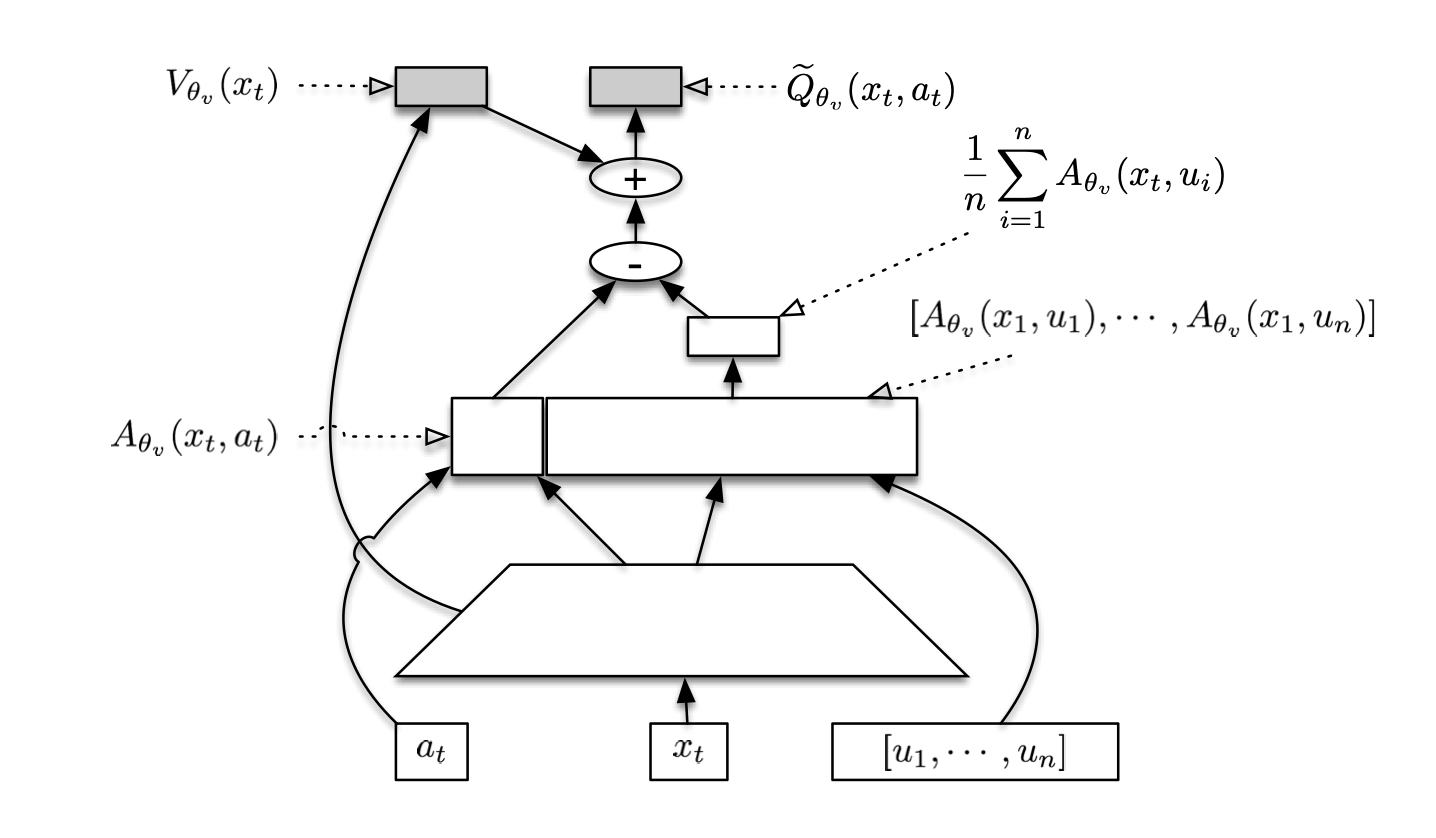
\includegraphics[scale=0.5, width=\textwidth]{SDN.png}
\end{figure}

For the continuous case, since it is unpractical to compute value by summing up the action-values, 
we should deterministically get output from the critic network.
To acheive this, the paper uses a Stochastic Dueling Network(SDN) to estimate both $V^\pi$ and $Q^\pi$
while maintaining consistency between two estimates.(see Figure 1)

The corresponding estimate for $Q^\pi$ of SDN is computed as follows:
\[
  \tilde{Q}_{\theta_v}(x_t, a_t) \sim V_{\theta_v}(x_t) + A_{\theta_v}(x_t, a_t) - \frac{1}{n}\sum_{i = 1}^n A_{\theta_v}(x_t, u_i), \text{where } u_i \sim \pi(\cdot | x_t)
\]
To train the network, the paper as well uses $Q^{ret}$ for target action-value.
For the state value $V^\pi$, they uses the following target:
\[
    V^{target}(x_t) = \min\{1, \frac{\pi(a_t|x_t)}{\mu(a_t | x_t)}\} (Q^{ret}(x_t, a_t) - V_{\theta_v}(x_t))
\]
, which is derived by applying the trunction and bias correction trick like what have been done on the policy gradient update.

For continous trust region updating, the paper replaced $Q^{ret}$ with $Q^{opc}$, 
which is basically $Q^{ret}$ without truncated importance ratio.
Though might resulting in a less stable learning, $Q^{opc}$ could better utilize the returns since its not truncated.
The choice is made since by experiment they found out that $Q^{opc}$ often leads to faster learning on continous cases.


\section{Detailed Implementation}
\label{section:implementation}
Please explain your implementation in detail. You may do this with the help of pseudo code or a figure of system architecture. Please also highlight which parts of the algorithm lead to the most difficulty in your implementation.


As for the part of ablations, we conduct the following alterations. 

\begin{enumerate}
    \item remove the entropy term
    \item remove \emph{trust region constraint}
    \item drop the bias term 
    \item remove the clamping on the actor loss
    \item change the \emph{truncation parameter}
    \item change $Q_opc$ to $Q_ret$ 
    \item change $Q_ret$ to $Q_opc$
    \item change the power term of truncated importance weight from $1/d$ to $1 / e^d$
    \item replace sdn structure to two independent networks
\end{enumerate}


1~5 are conducted under both discrete and continuous environments, while 6~9 are only considered under continuous environment.
\begin{enumerate}
    \item Remove the entropy term 
    As we can see, when we remove the entropy term, the performane will get worse. 
    \item Remove trust region constraint\\
    In the environment of CartPole and MountainCarContinuous, the removal of trust region constraint from the algorithm seems to be better, especially in the MountainCarContinuous environment. 
    \item Drop the bias term\\
    In both environment, the result with bias term dropped turns out to be significantly worse. 
    \item Remove the clamping on the actor loss\\
    In both environments, the result gets worse after we remove the clamping function. The reward would change slightly after certain episodes.
    \item Change the truncation parameter\\
    It appears that the results of each corresponding hyperparameters are almost the same in the last few episodes. 
    \item Change Qopc to Qret\\
    The result is worse after we conduct the state-action value replacement.
    \item Change Qret to Qopc\\
    The result is also worse after we conduct the state-action value replacement. Moreover, the reward would remain unchanged after some episodes.
    \item Change the power term of truncated importance weight from $1/d$ to $1/e^d$\\
    The change leads to a better performane, since d is the dimensionality of the action space. The alteration causes smaller truncated importane weight.
    \item Replace sdn structure to two independent networks\\
    The result gets worse after replacing the original network to two independent networks. The reward would change slightly after certain episodes.
\end{enumerate}


\section{Empirical Evaluation}
\label{section:evaluation}
Please showcase your empirical results in this section. Please clearly specify which sets of experiments of the original paper are considered in your report. Please also report the corresponding hyperparameters of each experiment.


1. remove the entropy term

2. consider the parameter TRUST_REGION_CONSTRAINT
3. drop the bias term 
4. remove the clamping on the actor loss
5. change the truncation parameter
6. change Q_opc to Q_ret 
7. change Q_ret to Q_opc
8. change the power term of truncated importance weight from 1/d to 1 / e^d 
9. replace sdn structure to two independent networks


\begin{figure}
\caption{clamp the actor loss under continuous}
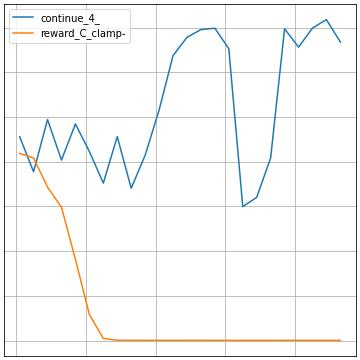
\includegraphics[scale=0.5, width=\textwidth]{continuous/clamp.jpg}
\end{figure}
    

\section{Conclusion}
\label{section:conclusion}
Please provide succinct concluding remarks for your report. You may discuss the following aspects:
\begin{itemize}
    \item The potential future research directions
    \item Any technical limitations
    \item Any latest results on the problem of interest
\end{itemize}



{
  \small
  \bibliographystyle{unsrtnat}
  \bibliography{reference}
}

\end{document}
